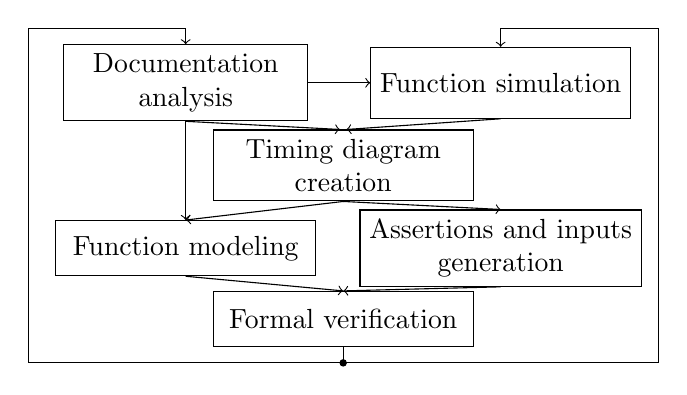
\begin{tikzpicture}[->, node distance=1cm,connection/.style={draw,circle,fill=black,inner sep=0.8pt}]

  \node[rectangle, draw, minimum width=3.1cm, minimum height=.9cm, align=center](documentation) at (0,0){Documentation\\analysis};
  \node[rectangle, draw, minimum width=3.1cm, minimum height=.9cm, align=center](simulation) at (4,0){Function simulation};
  \node[rectangle, draw, minimum width=3.3cm, minimum height=.9cm, align=center](time) at (2,-1.05){Timing diagram\\creation};
  \node[rectangle, draw, minimum width=3.3cm, minimum height=.7cm, align=center](assertions) at (4,-2.1){Assertions and inputs\\generation};
  \node[rectangle, draw, minimum width=3.3cm, minimum height=.7cm, align=center](modeling) at (0,-2.1){Function modeling};
  \node[rectangle, draw, minimum width=3.3cm, minimum height=.7cm, align=center](verification) at (2,-3){Formal verification};

  \draw[->] (documentation.east) -- (simulation.west);
  \draw[->] (documentation.south) -- (time.95);
  \draw[->] (documentation.south) -- (modeling.north);
  \draw[->] (simulation.south) -- (time.85);
  \draw[->] (time.south) -- (assertions.north);
  \draw[->] (assertions.south) -- (verification.north);
  \draw[->] (time.south) -- (modeling.north);
  \draw[->] (modeling.south) -- (verification.north);

  \draw[-] (verification.south) --++(0,-.2) node[connection,pos=1]{};
  \draw[->] (verification.south)++(0,-.2) --++(4,0) --++(0,4.25) -| (simulation.north); 
  \draw[->] (verification.south)++(0,-.2) --++(-4,0) --++(0,4.25) -| (documentation.north); 
       
\end{tikzpicture}